\documentclass[11pt,a4paper]{article}

% =============================================================================
% PACKAGES
% =============================================================================
\usepackage[utf8]{inputenc}
\usepackage[T1]{fontenc}
\usepackage{geometry}
\geometry{margin=2.5cm}

% Graphics and figures
\usepackage{graphicx}
\usepackage{float}
\usepackage{subcaption}
\graphicspath{{figures/}}

% Tables
\usepackage{booktabs}
\usepackage{tabularx}
\usepackage{multirow}

% Math
\usepackage{amsmath}
\usepackage{amssymb}

% References and links
\usepackage{hyperref}
\hypersetup{
    colorlinks=true,
    linkcolor=blue,
    citecolor=blue,
    urlcolor=blue
}

% Bibliography
\usepackage{natbib}
\bibliographystyle{apalike}

% Code listings (for methods documentation)
\usepackage{listings}
\lstset{
    basicstyle=\ttfamily\small,
    breaklines=true,
    frame=single,
    language=Python
}

% Colors for highlighting
\usepackage{xcolor}
\definecolor{observation}{RGB}{39,174,96}
\definecolor{finding}{RGB}{41,128,185}
\definecolor{todo}{RGB}{231,76,60}

% Custom commands for annotations
\newcommand{\observation}[1]{\textcolor{observation}{\textbf{[OBS:} #1\textbf{]}}}
\newcommand{\finding}[1]{\textcolor{finding}{\textbf{[FIND:} #1\textbf{]}}}
\newcommand{\todo}[1]{\textcolor{todo}{\textbf{[TODO:} #1\textbf{]}}}

% =============================================================================
% DOCUMENT INFO
% =============================================================================
\title{Semantic Clustering of Agricultural Drone Imagery\\Using Vision-Language Embeddings}
\author{Research Notes - Draft v0.1}
\date{January 2026 \\ \small Last updated: \today}

% =============================================================================
% DOCUMENT
% =============================================================================
\begin{document}

\maketitle

\begin{abstract}
% =============================================================================
% ABSTRACT
% Status: DRAFT - To be refined
% =============================================================================

This study explores the application of vision-language embedding models for automatic semantic categorization of agricultural drone imagery. Using CLIP (Contrastive Language-Image Pre-training) embeddings with UMAP dimensionality reduction, we demonstrate that drone survey images can be automatically clustered by semantic content---specifically by flight altitude and imaging purpose---without manual labeling. Analysis of 97 drone images from a tomato field survey in Santa Ines, Chile reveals two distinct clusters: close-up crop inspection images (92\%) and high-altitude field mapping images (8\%). Similarity network analysis confirms strong cluster cohesion with only 2.7\% cross-category connections. These findings suggest that pretrained vision-language models offer a promising approach for organizing and filtering large agricultural drone datasets, potentially reducing manual curation effort in precision agriculture workflows.

\todo{Refine abstract after completing results section}

\end{abstract}

\tableofcontents
\newpage

% -----------------------------------------------------------------------------
\section{Introduction}
\label{sec:introduction}
% =============================================================================
% INTRODUCTION
% Status: DRAFT - Framework established, needs literature review
% =============================================================================

\subsection{Background}

Unmanned Aerial Vehicles (UAVs) have become essential tools in precision agriculture, enabling high-resolution monitoring of crop health, irrigation patterns, and field conditions. Modern drone surveys generate large volumes of imagery---often hundreds to thousands of images per flight session---creating significant data management challenges.

\todo{Add citations: drone imagery in agriculture, data volume challenges}

A typical agricultural drone survey may include:
\begin{itemize}
    \item \textbf{Systematic mapping flights}: High-altitude images for orthomosaic generation
    \item \textbf{Targeted inspection flights}: Low-altitude close-ups of specific crop areas
    \item \textbf{Oblique/transitional images}: Various angles during ascent/descent
\end{itemize}

Organizing this heterogeneous imagery typically requires manual review or relies solely on GPS metadata, which captures \emph{where} images were taken but not \emph{what} they contain semantically.

\subsection{Vision-Language Models for Image Understanding}

Recent advances in vision-language models, particularly CLIP (Contrastive Language-Image Pre-training), have demonstrated remarkable zero-shot capabilities for image understanding. These models learn joint embeddings of images and text, enabling semantic similarity comparisons without task-specific training.

\observation{CLIP embeddings capture semantic content (altitude/purpose) rather than just spatial position---this is a key distinction from GPS-based organization}

\subsection{Research Gap}

While vision-language models have been extensively studied for general image classification and retrieval, their application to agricultural drone imagery organization remains underexplored. Specifically:

\begin{enumerate}
    \item Can pretrained models (without agricultural fine-tuning) meaningfully cluster drone imagery?
    \item What semantic distinctions do these models capture in agricultural contexts?
    \item How do embedding-based clusters compare to traditional metadata-based organization?
\end{enumerate}

\todo{Expand literature review: existing work on drone image organization, CLIP applications in remote sensing}


% -----------------------------------------------------------------------------
\section{Objectives}
\label{sec:objectives}
% =============================================================================
% OBJECTIVES
% Status: DRAFT - Core objectives defined
% =============================================================================

\subsection{General Objective}

To evaluate the effectiveness of vision-language embedding models for automatic semantic organization of agricultural drone imagery, with application to precision agriculture data management workflows.

\subsection{Specific Objectives}

\begin{enumerate}
    \item \textbf{Embedding Analysis}: Compute and visualize CLIP embeddings for drone survey imagery to identify natural semantic clusters.

    \item \textbf{Cluster Characterization}: Analyze the semantic distinctions captured by embedding-based clusters (e.g., altitude, crop visibility, image purpose).

    \item \textbf{Comparison with Metadata}: Compare embedding-based organization with GPS/EXIF metadata-based approaches to understand complementary information.

    \item \textbf{Similarity Search}: Implement and evaluate content-based image retrieval for finding similar drone images within large datasets.

    \item \textbf{Workflow Integration}: Develop practical tools for integrating embedding-based organization into agricultural data pipelines.
\end{enumerate}

\subsection{Hypotheses}

\begin{description}
    \item[H1] Pretrained CLIP embeddings will separate drone images by semantic content (flight altitude, imaging purpose) without domain-specific training.

    \item[H2] Embedding-based clusters will capture information orthogonal to GPS position---images from different locations but similar purposes will cluster together.

    \item[H3] Similarity search based on embeddings will retrieve semantically relevant images more effectively than spatial proximity alone.
\end{description}

\todo{Refine hypotheses based on preliminary results}


% -----------------------------------------------------------------------------
\section{Materials and Methods}
\label{sec:methods}
% =============================================================================
% MATERIALS AND METHODS
% Status: DRAFT - Core methodology documented
% =============================================================================

\subsection{Study Area and Data Collection}

\subsubsection{Location}
Santa Ines agricultural field, Chile. Tomato cultivation site monitored via drone surveys.

\todo{Add exact coordinates, field size, crop details}

\subsubsection{Drone Imagery Dataset}
\begin{itemize}
    \item \textbf{Platform}: DJI drone (model TBD)
    \item \textbf{Image count}: 97 images
    \item \textbf{File format}: JPEG, approximately 10-12 MB per image
    \item \textbf{Resolution}: High-resolution (dimensions TBD from metadata)
    \item \textbf{Date}: January 2026
\end{itemize}

\subsection{Software Environment}

\subsubsection{Dataset Management}
FiftyOne v1.12.0 \citep{fiftyone} was used for dataset management, embedding computation, and visualization. FiftyOne provides:
\begin{itemize}
    \item Efficient handling of large image datasets
    \item Built-in integration with embedding models
    \item Interactive visualization tools
    \item Similarity search functionality
\end{itemize}

\subsubsection{Analysis Tools}
\begin{itemize}
    \item \textbf{Python 3.12}: Data processing and embedding computation
    \item \textbf{R 4.3.3}: Statistical analysis and visualization (ggplot2)
    \item \textbf{PyTorch}: Deep learning backend for CLIP model
\end{itemize}

\subsection{Embedding Computation}

\subsubsection{Model Selection}
CLIP ViT-B/32 (Vision Transformer, Base, 32x32 patches) was selected for embedding computation. This model:
\begin{itemize}
    \item Provides 512-dimensional embeddings per image
    \item Was pretrained on 400M image-text pairs
    \item Offers good balance of computational efficiency and semantic richness
\end{itemize}

\subsubsection{Dimensionality Reduction}
UMAP (Uniform Manifold Approximation and Projection) was applied to reduce embeddings from 512D to 2D for visualization:

\begin{equation}
    \mathbf{z}_i = \text{UMAP}(\mathbf{e}_i), \quad \mathbf{e}_i \in \mathbb{R}^{512}, \quad \mathbf{z}_i \in \mathbb{R}^{2}
\end{equation}

\todo{Add UMAP hyperparameters: n\_neighbors, min\_dist, metric}

\subsubsection{Implementation}
\begin{lstlisting}[language=Python, caption=Embedding computation with FiftyOne]
import fiftyone as fo
import fiftyone.brain as fob

dataset = fo.load_dataset("santa_ines_dron")

# Compute CLIP embeddings with UMAP projection
fob.compute_visualization(
    dataset,
    brain_key="clip_viz",
    model="clip-vit-base32-torch",
    method="umap"
)

# Compute similarity index for retrieval
fob.compute_similarity(
    dataset,
    brain_key="clip_similarity",
    embeddings="clip_viz"
)
\end{lstlisting}

\subsection{Clustering and Classification}

Image clusters were identified through visual inspection of the UMAP projection. Two distinct clusters emerged:

\begin{enumerate}
    \item \textbf{Main cluster} (89 images): Concentrated in UMAP region $x \in [6.8, 10.5]$, $y \in [0.5, 4.5]$
    \item \textbf{Outlier cluster} (8 images): Isolated at $x \approx 11.5$, $y \approx -0.7$
\end{enumerate}

Images were tagged based on cluster membership for subsequent analysis.

\subsection{Similarity Network Analysis}

To quantify cluster structure, a k-nearest neighbor graph was constructed:

\begin{itemize}
    \item Each image connected to its $k=3$ nearest neighbors in embedding space
    \item Distance metric: Euclidean distance in 2D UMAP space
    \item Edge classification: within-category vs. cross-category connections
\end{itemize}

\subsection{Statistical Analysis}

Cluster cohesion was evaluated using:
\begin{itemize}
    \item Mean distance to $k$ nearest neighbors
    \item Inter-cluster centroid distance
    \item Proportion of cross-category edges in similarity network
\end{itemize}

All statistical analyses and visualizations were performed in R using ggplot2.


% -----------------------------------------------------------------------------
\section{Results}
\label{sec:results}
% =============================================================================
% RESULTS
% Status: DRAFT - Initial results documented
% =============================================================================

\subsection{Combined Spatial and Visual Analysis}

Figure~\ref{fig:combined} presents an integrated view of the Santa Ines drone survey analysis, demonstrating the fundamental difference between physical GPS locations and visual semantic clustering.

\begin{figure}[H]
    \centering
    
\includegraphics[width=\textwidth]{combined_analysis.png}
    \caption{Combined analysis of Santa Ines drone imagery. \textbf{(A)} GPS coordinates overlaid on satellite imagery showing flight coverage; \textbf{(B)} UMAP projection of CLIP embeddings revealing two semantic clusters; \textbf{(C)} Representative close-up images capturing detailed crop inspection views; \textbf{(D)} Representative high-altitude overview images showing vineyard row patterns.}
    \label{fig:combined}
\end{figure}

\subsubsection{GPS vs Visual Embedding: Key Differences}

Panel A reveals the physical flight pattern over the Santa Ines vineyard. The drone followed systematic transects across the crop rows, with close-up images (green markers) distributed along parallel flight lines and high-altitude overview images (red markers) captured at strategic positions across the field. Geographically, both image types are \textbf{spatially intermixed}---high-altitude shots were taken from various positions throughout the survey area.

In contrast, Panel B shows the CLIP embedding space where images cluster by \textbf{visual content rather than geographic location}. Despite being captured from scattered GPS positions, all high-altitude images form a tight cluster in the lower-right corner of the embedding space, clearly separated from the close-up images. This demonstrates that vision-language models organize images by semantic similarity (what the image depicts) rather than spatial proximity (where it was captured).

\subsubsection{Visual Characteristics of Each Cluster}

Panels C and D provide visual evidence for why CLIP separates these image categories:

\textbf{Close-up images (Panel C)} are characterized by:
\begin{itemize}
    \item High detail of individual vine plants and foliage
    \item Visible leaf texture, color variations, and plant structure
    \item Limited field-of-view showing 1-3 plant rows
    \item Rich color palette dominated by greens and earth tones
\end{itemize}

\textbf{High-altitude images (Panel D)} exhibit distinct visual patterns:
\begin{itemize}
    \item Geometric vineyard row patterns visible from above
    \item Uniform texture showing repetitive agricultural structure
    \item Wide field-of-view capturing dozens of rows
    \item Reduced color variation with dominant green/brown striping
\end{itemize}

\finding{CLIP embeddings successfully capture the semantic distinction between ``detailed crop inspection'' and ``field overview'' image types, enabling automatic categorization based purely on visual content}

\observation{This spatial-semantic decoupling has practical implications: images can be organized by content type regardless of capture location, enabling more intuitive dataset browsing and quality control workflows}

\subsection{Embedding Space Visualization}

CLIP embeddings projected to 2D via UMAP revealed two distinct clusters in the Santa Ines drone dataset (Figure~\ref{fig:embeddings}).

\begin{figure}[H]
    \centering
    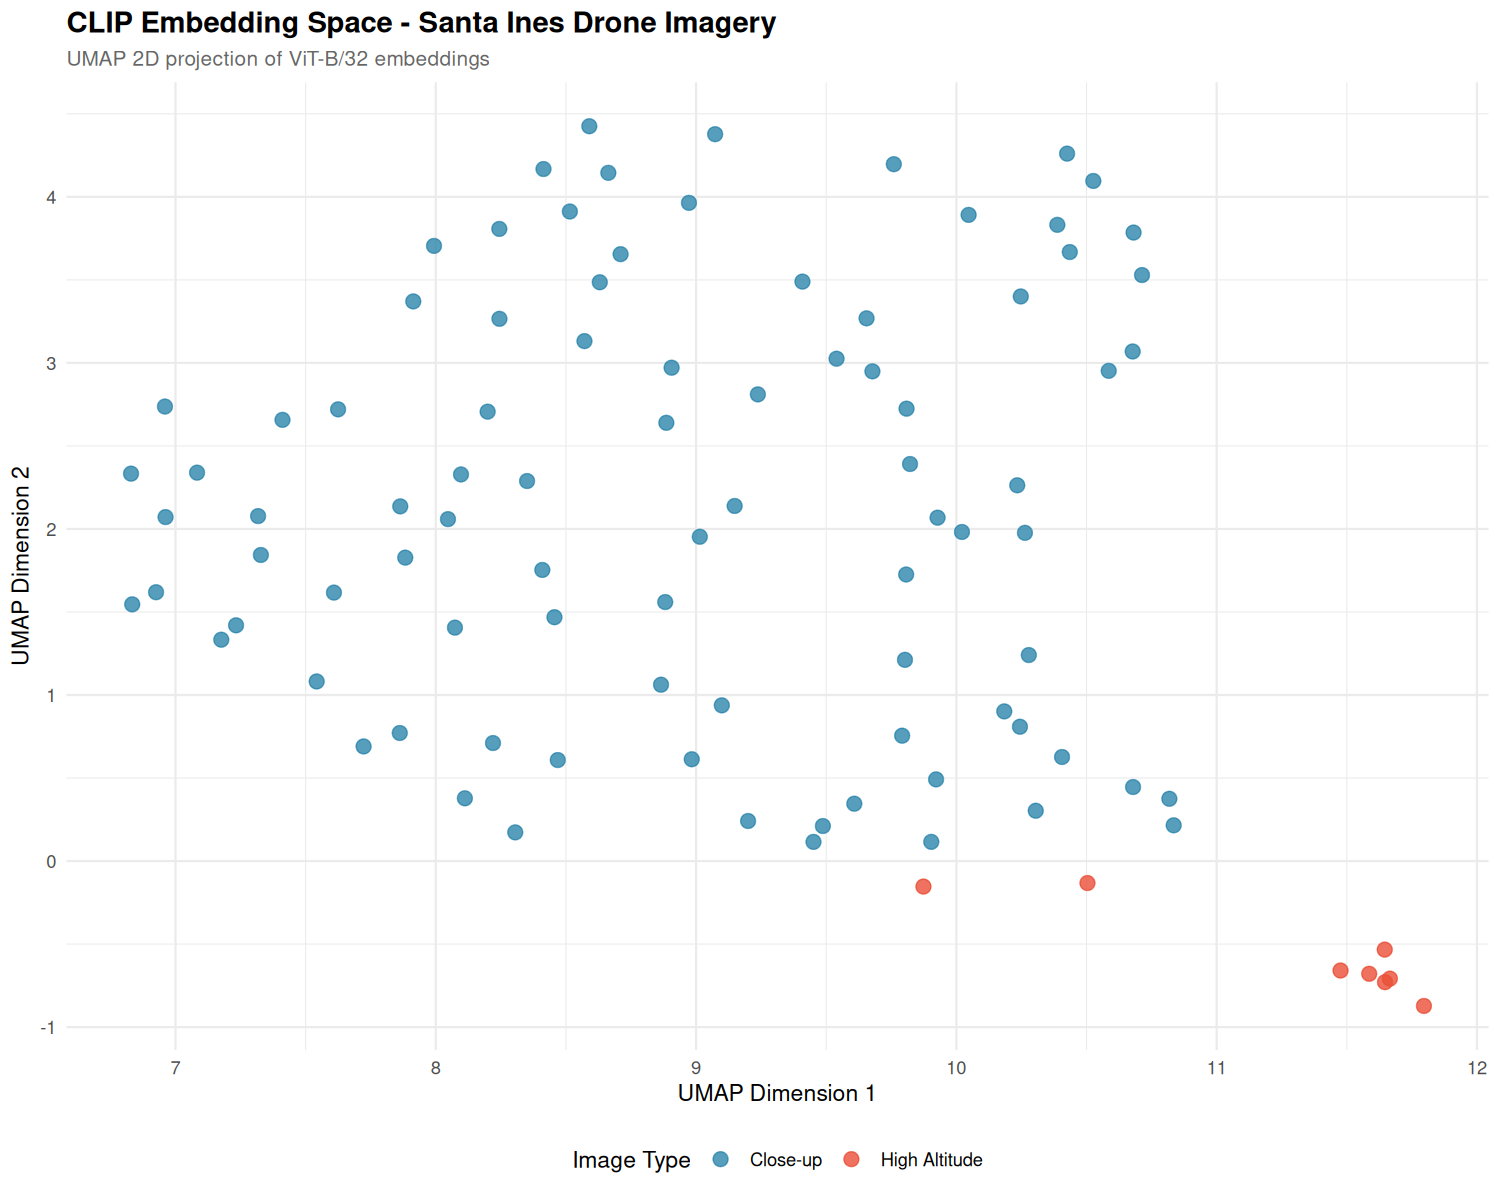
\includegraphics[width=0.9\textwidth]{r_embeddings_plot.png}
    \caption{UMAP projection of CLIP embeddings for 97 drone images. Blue points represent close-up crop inspection images; red points represent high-altitude overview images.}
    \label{fig:embeddings}
\end{figure}

\subsubsection{Cluster Characteristics}

\begin{table}[H]
\centering
\caption{Summary statistics for identified image clusters}
\label{tab:clusters}
\begin{tabular}{lcccc}
\toprule
\textbf{Category} & \textbf{Count} & \textbf{Percentage} & \textbf{UMAP X (mean $\pm$ sd)} & \textbf{UMAP Y (mean $\pm$ sd)} \\
\midrule
Close-up (crop inspection) & 89 & 91.8\% & $8.97 \pm 1.15$ & $2.15 \pm 1.28$ \\
High-altitude (overview) & 8 & 8.2\% & $11.30 \pm 0.70$ & $-0.56 \pm 0.27$ \\
\bottomrule
\end{tabular}
\end{table}

\observation{The high-altitude cluster shows lower variance (tighter grouping), suggesting more homogeneous visual content among overview images}

\subsubsection{Inter-cluster Distance}

The Euclidean distance between cluster centroids in UMAP space was \textbf{3.56 units}, indicating clear separation between semantic categories.

\subsection{Similarity Network Structure}

Network analysis of the 3-nearest-neighbor graph revealed strong within-cluster connectivity (Figure~\ref{fig:network}).

\begin{figure}[H]
    \centering
    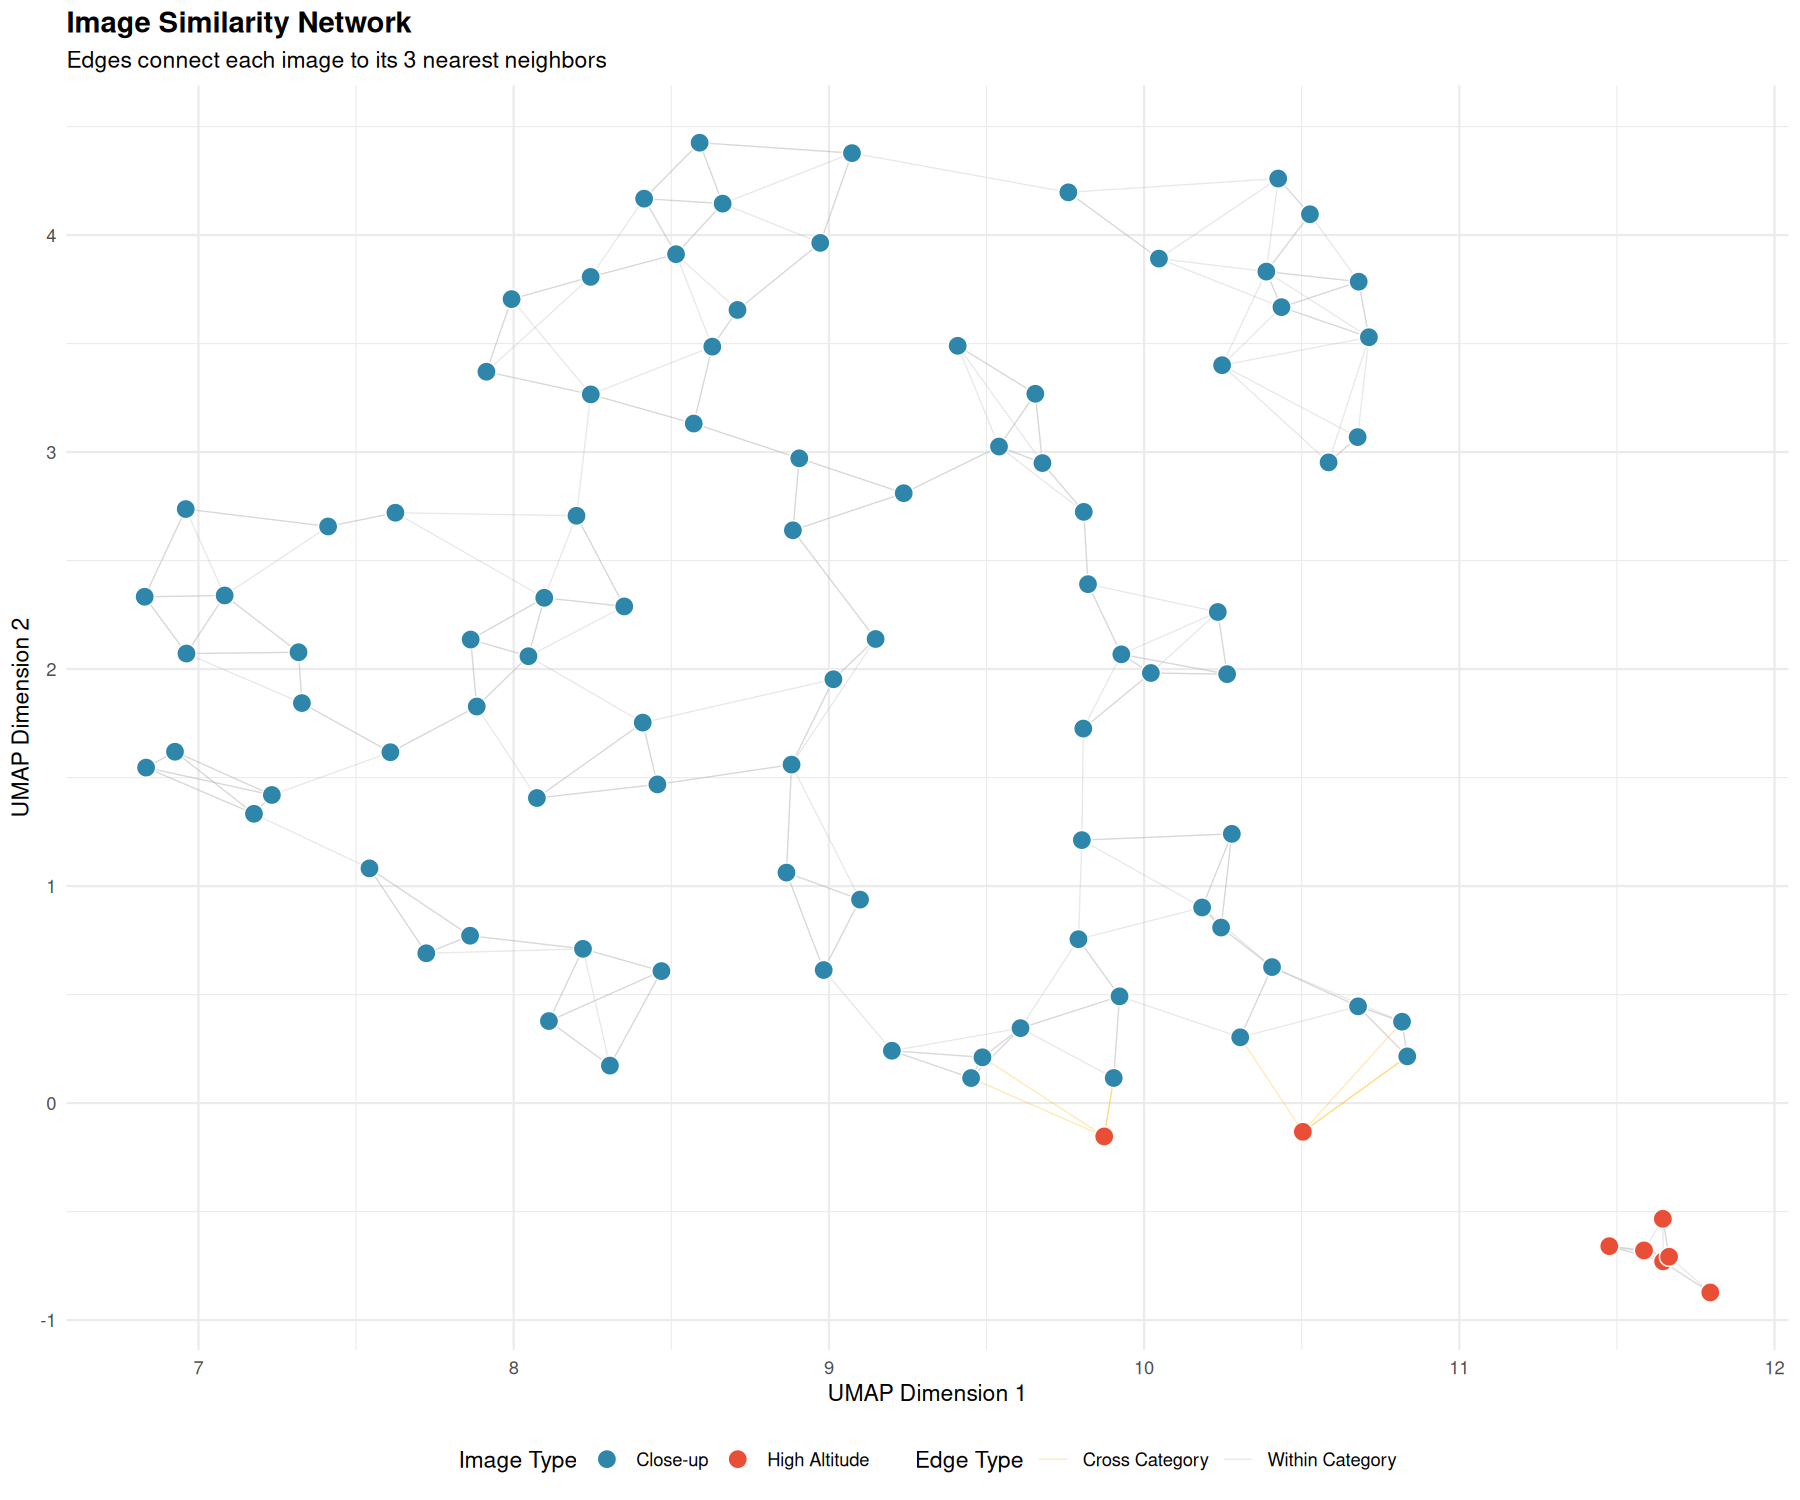
\includegraphics[width=0.95\textwidth]{r_similarity_network.png}
    \caption{Image similarity network. Nodes represent images (blue = close-up, red = high-altitude). Gray edges connect images within the same category; yellow edges indicate cross-category connections.}
    \label{fig:network}
\end{figure}

\subsubsection{Network Statistics}

\begin{itemize}
    \item \textbf{Total edges}: 291 (3 per image $\times$ 97 images)
    \item \textbf{Within-category edges}: 283 (97.3\%)
    \item \textbf{Cross-category edges}: 8 (2.7\%)
\end{itemize}

\finding{Only 2.7\% of nearest-neighbor connections cross category boundaries, confirming robust cluster separation}

\subsection{Cluster Cohesion Analysis}

Mean distance to 5 nearest neighbors was computed for each category (Figure~\ref{fig:cohesion}).

\begin{figure}[H]
    \centering
    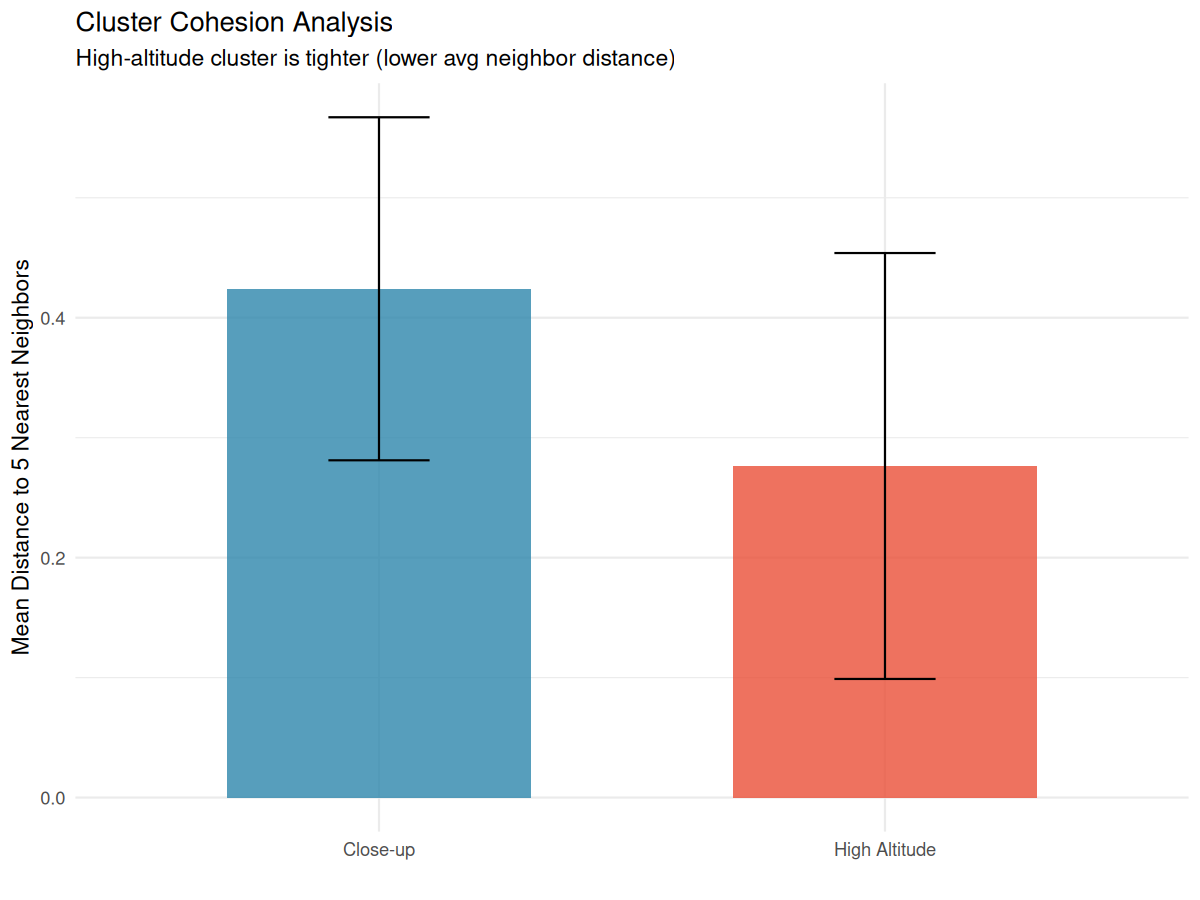
\includegraphics[width=0.7\textwidth]{r_cluster_cohesion.png}
    \caption{Cluster cohesion measured by mean distance to 5 nearest neighbors. Error bars show standard deviation.}
    \label{fig:cohesion}
\end{figure}

\begin{table}[H]
\centering
\caption{Cluster cohesion statistics}
\label{tab:cohesion}
\begin{tabular}{lccc}
\toprule
\textbf{Category} & \textbf{Mean Distance} & \textbf{Std Dev} & \textbf{n (neighbor pairs)} \\
\midrule
Close-up & 0.424 & 0.143 & 445 \\
High-altitude & 0.276 & 0.178 & 40 \\
\bottomrule
\end{tabular}
\end{table}

\observation{High-altitude cluster is 35\% more cohesive (lower neighbor distance) than the close-up cluster, despite having fewer samples}

\subsection{Image Size Analysis}

File size distribution showed modest differences between categories (Figure~\ref{fig:size}).

\begin{figure}[H]
    \centering
    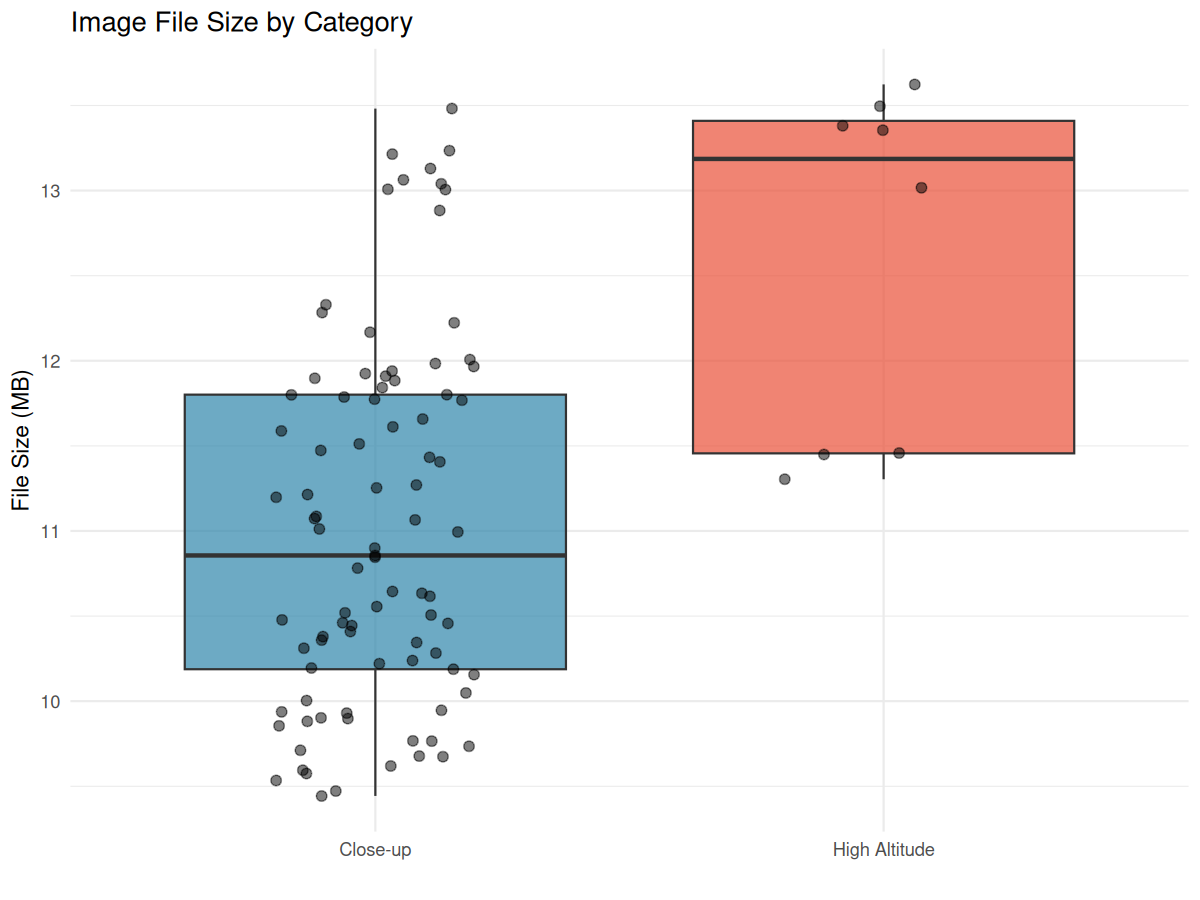
\includegraphics[width=0.7\textwidth]{r_size_analysis.png}
    \caption{Distribution of image file sizes by category.}
    \label{fig:size}
\end{figure}

\begin{itemize}
    \item Close-up images: mean 11.0 MB
    \item High-altitude images: mean 12.6 MB
\end{itemize}

\subsection{Similarity Search Validation}

Content-based image retrieval was tested using high-altitude images as queries. Results confirm that similarity search returns semantically consistent results:

\begin{table}[H]
\centering
\caption{Top-5 similar images for query DJI\_0552.JPG (high-altitude)}
\label{tab:similarity}
\begin{tabular}{clc}
\toprule
\textbf{Rank} & \textbf{Image} & \textbf{Category} \\
\midrule
1 & DJI\_0552.JPG & High-altitude (query) \\
2 & DJI\_0557.JPG & High-altitude \\
3 & DJI\_0555.JPG & High-altitude \\
4 & DJI\_0556.JPG & High-altitude \\
5 & DJI\_0554.JPG & High-altitude \\
\bottomrule
\end{tabular}
\end{table}

\finding{All top-5 results for a high-altitude query are also high-altitude images, demonstrating effective semantic retrieval}


% -----------------------------------------------------------------------------
\section{Discussion}
\label{sec:discussion}
% =============================================================================
% DISCUSSION
% Status: DRAFT - Initial interpretation, needs expansion
% =============================================================================

\subsection{Interpretation of Results}

\subsubsection{Semantic Clustering Without Domain-Specific Training}

The most significant finding is that CLIP embeddings---trained on general web images, not agricultural data---successfully separated drone images by their functional purpose (inspection vs. mapping). This suggests that:

\begin{enumerate}
    \item Pretrained vision-language models capture transferable visual concepts
    \item Altitude-related visual features (scale, detail level, field-of-view) are well-represented in general visual embeddings
    \item Domain-specific fine-tuning may not be necessary for basic organizational tasks
\end{enumerate}

\observation{CLIP's training on diverse web data appears to include sufficient exposure to aerial/satellite imagery to enable meaningful agricultural drone image understanding}

\subsubsection{Embedding Space vs. Geographic Space}

A key advantage of embedding-based organization over GPS metadata is the capture of \emph{semantic} rather than \emph{spatial} similarity. Images taken at different GPS locations but serving the same purpose (e.g., all high-altitude mapping shots) cluster together in embedding space, whereas GPS coordinates would scatter them across the field.

\todo{Add quantitative comparison: GPS clustering vs. embedding clustering}

\subsubsection{Cluster Cohesion Asymmetry}

The high-altitude cluster showed higher cohesion (lower mean neighbor distance) than the close-up cluster. This may reflect:

\begin{itemize}
    \item \textbf{Homogeneity of overview images}: High-altitude shots capture similar field patterns regardless of position
    \item \textbf{Diversity of inspection targets}: Close-up images may show varied crop conditions, growth stages, or inspection targets
\end{itemize}

\finding{Cluster cohesion differences may indicate semantic diversity within categories---useful for quality assessment or anomaly detection}

\subsection{Practical Implications}

\subsubsection{Automated Dataset Curation}

The demonstrated clustering capability enables automated organization of drone survey data:

\begin{itemize}
    \item Separate mapping images from inspection images automatically
    \item Identify outliers or unusual images for review
    \item Filter large datasets to specific image types without manual labeling
\end{itemize}

\subsubsection{Content-Based Image Retrieval}

Similarity search based on embeddings provides intuitive ``find similar'' functionality:

\begin{itemize}
    \item Query by example: find all images similar to a selected sample
    \item Batch processing: process only images of a specific type
    \item Quality control: identify near-duplicates or redundant coverage
\end{itemize}

\subsection{Limitations}

\begin{enumerate}
    \item \textbf{Sample size}: Analysis based on 97 images from a single field; generalization requires validation on larger, more diverse datasets

    \item \textbf{Binary clustering}: Current analysis identified only two categories; finer-grained distinctions (e.g., crop health categories) were not explored

    \item \textbf{UMAP projection}: 2D visualization may lose information present in the full 512D embedding space

    \item \textbf{Model selection}: Only CLIP ViT-B/32 was evaluated; other models may perform differently
\end{enumerate}

\todo{Address limitations in future work section}

\subsection{Comparison with Related Work}

\todo{Add comparison with existing drone image organization methods, GPS-based clustering, traditional image classification approaches}

\subsection{Future Directions}

\begin{enumerate}
    \item \textbf{Multi-field validation}: Apply methodology to datasets from multiple agricultural sites
    \item \textbf{Fine-grained classification}: Explore embeddings for crop health assessment, disease detection
    \item \textbf{Temporal analysis}: Track embedding changes across growing season
    \item \textbf{Model comparison}: Evaluate agricultural-specific models vs. general pretrained models
\end{enumerate}


% -----------------------------------------------------------------------------
\section{Conclusions}
\label{sec:conclusions}
% =============================================================================
% CONCLUSIONS
% Status: DRAFT - Summary of key findings
% =============================================================================

This study demonstrated that pretrained vision-language embeddings (CLIP) effectively organize agricultural drone imagery by semantic content without domain-specific training. Key findings include:

\begin{enumerate}
    \item \textbf{Automatic clustering}: CLIP embeddings with UMAP projection separated 97 drone images into two semantically meaningful clusters: close-up crop inspection (89 images, 92\%) and high-altitude field mapping (8 images, 8\%).

    \item \textbf{Strong cluster separation}: Only 2.7\% of nearest-neighbor connections crossed category boundaries, indicating robust semantic clustering.

    \item \textbf{Effective similarity search}: Content-based image retrieval correctly identified semantically similar images, enabling intuitive ``find similar'' functionality.

    \item \textbf{Complementary to GPS}: Embedding-based organization captures semantic similarity (image purpose) orthogonal to spatial position captured by GPS metadata.
\end{enumerate}

These results suggest that pretrained vision-language models offer a practical, zero-configuration approach for organizing large agricultural drone datasets. By reducing manual curation effort, this methodology can accelerate precision agriculture workflows and enable more efficient use of drone survey data.

\todo{Refine conclusions after completing discussion section}


% -----------------------------------------------------------------------------
% APPENDICES
\appendix
\section{Observation Log}
\label{app:observations}
% =============================================================================
% OBSERVATION LOG
% Status: ACTIVE - Updated throughout research process
% =============================================================================

% This appendix maintains a chronological log of observations made during
% the research process. Observations are tagged with dates and linked to
% relevant figures/sections where applicable.

\subsection*{Log Format}
Each observation entry includes:
\begin{itemize}
    \item \textbf{Date}: When the observation was made
    \item \textbf{Category}: Type of observation (data, method, result, idea)
    \item \textbf{Description}: The observation itself
    \item \textbf{Link}: Reference to relevant section, figure, or data
\end{itemize}

\hrulefill

\subsection*{2026-01-13}

\begin{description}
    \item[OBS-001] \textbf{[Data]} Dataset loaded successfully: 97 DJI drone images from Santa Ines field, ~10-12 MB each.

    \item[OBS-002] \textbf{[Result]} UMAP projection reveals clear bimodal structure---main cluster of 89 images and outlier cluster of 8 images at bottom-right of embedding space.

    \item[OBS-003] \textbf{[Result]} Outlier images (DJI\_0469, DJI\_0509, DJI\_0552-0557) visually confirmed as high-altitude overview shots, distinct from close-up crop inspection images.

    \item[OBS-004] \textbf{[Method]} CLIP embeddings capture altitude/scale differences effectively---semantic clustering emerges without altitude metadata being provided.
\end{description}

\subsection*{2026-01-14}

\begin{description}
    \item[OBS-005] \textbf{[Result]} Similarity index computed successfully. Query tests confirm semantically consistent retrieval---high-altitude queries return only high-altitude neighbors.

    \item[OBS-006] \textbf{[Result]} Network analysis: 97.3\% of k-NN edges stay within category. Only 8/291 edges cross category boundary.

    \item[OBS-007] \textbf{[Result]} Cluster cohesion asymmetry: high-altitude cluster is 35\% tighter (mean neighbor distance 0.276 vs 0.424). May indicate greater visual homogeneity of overview shots.

    \item[OBS-008] \textbf{[Idea]} Cohesion metric could serve as diversity indicator---tight clusters = homogeneous content, diffuse clusters = varied content. Useful for coverage assessment.

    \item[OBS-009] \textbf{[Method]} R/ggplot2 workflow established for reproducible analysis. Scripts: \texttt{analysis.R}, \texttt{similarity\_analysis.R}.
\end{description}

\hrulefill

\subsection*{Template for Future Entries}

\begin{description}
    \item[OBS-XXX] \textbf{[Category]} Description of observation. \textit{See Section~X / Figure~X}
\end{description}

% =============================================================================
% OBSERVATION INDEX BY CATEGORY
% =============================================================================

\subsection*{Index by Category}

\textbf{Data observations:} OBS-001

\textbf{Method observations:} OBS-004, OBS-009

\textbf{Result observations:} OBS-002, OBS-003, OBS-005, OBS-006, OBS-007

\textbf{Ideas/hypotheses:} OBS-008


\section{Technical Details}
\label{app:technical}
% =============================================================================
% TECHNICAL DETAILS
% Status: Reference documentation
% =============================================================================

\subsection{Software Versions}

\begin{table}[H]
\centering
\begin{tabular}{ll}
\toprule
\textbf{Software} & \textbf{Version} \\
\midrule
FiftyOne & 1.12.0 \\
Python & 3.12 \\
R & 4.3.3 \\
PyTorch & (system version) \\
CLIP model & ViT-B/32 \\
\bottomrule
\end{tabular}
\end{table}

\subsection{Data Paths}

\begin{verbatim}
research/
+-- paper/
|   +-- main.tex
|   +-- sections/
|   |   +-- abstract.tex
|   |   +-- introduction.tex
|   |   +-- objectives.tex
|   |   +-- methods.tex
|   |   +-- results.tex
|   |   +-- discussion.tex
|   |   +-- conclusions.tex
|   |   +-- observations.tex
|   |   +-- technical.tex
|   +-- figures/
+-- data/
|   +-- raw/
|   +-- processed/
|       +-- santa_ines_data.csv
|       +-- similarity_neighbors.csv
+-- analysis/
|   +-- R/
|   |   +-- analysis.R
|   |   +-- similarity_analysis.R
|   +-- python/
+-- notes/
+-- logs/
\end{verbatim}

\subsection{Key Commands}

\subsubsection{FiftyOne Dataset Operations}

\begin{lstlisting}[language=Python]
import fiftyone as fo
import fiftyone.brain as fob

# Load dataset
dataset = fo.load_dataset("santa_ines_dron")

# Access embeddings
results = dataset.load_brain_results("clip_viz")
points = results.points  # Shape: (97, 2)

# Similarity search
view = dataset.sort_by_similarity(
    sample_id, k=10, brain_key="clip_similarity"
)

# Filter by tags
high_alt = dataset.match_tags("high-altitude")
closeups = dataset.match_tags("close-up")
\end{lstlisting}

\subsubsection{Compilation}

\begin{lstlisting}[language=bash]
# Compile LaTeX document
cd research/paper
pdflatex main.tex
pdflatex main.tex  # Run twice for TOC

# Or use latexmk for automatic compilation
latexmk -pdf main.tex
\end{lstlisting}

\subsection{FiftyOne Brain Keys}

\begin{table}[H]
\centering
\begin{tabular}{lll}
\toprule
\textbf{Brain Key} & \textbf{Type} & \textbf{Description} \\
\midrule
clip\_viz & visualization & CLIP embeddings + UMAP 2D projection \\
clip\_similarity & similarity & Similarity index for retrieval \\
\bottomrule
\end{tabular}
\end{table}

\subsection{GPS Extraction from Drone Images}

GPS coordinates were extracted from EXIF metadata embedded in DJI drone images:

\begin{lstlisting}[language=Python]
from PIL import Image
from PIL.ExifTags import TAGS, GPSTAGS

def get_gps_coords(image_path):
    """Extract GPS coordinates from EXIF data"""
    image = Image.open(image_path)
    exif_data = image._getexif()

    gps_info = exif_data.get('GPSInfo', {})

    # Convert DMS to decimal degrees
    def to_degrees(dms):
        d, m, s = dms
        return d + m/60.0 + s/3600.0

    lat = to_degrees(gps_info['GPSLatitude'])
    if gps_info['GPSLatitudeRef'] == 'S':
        lat = -lat

    lon = to_degrees(gps_info['GPSLongitude'])
    if gps_info['GPSLongitudeRef'] == 'W':
        lon = -lon

    return lat, lon
\end{lstlisting}

\subsection{Satellite Map Integration}

Google Maps Static API was used to obtain satellite imagery background:

\begin{lstlisting}[language=Python]
import requests

API_KEY = "YOUR_API_KEY"
center_lat, center_lon = -34.4746, -70.9516
zoom = 18  # High zoom for agricultural detail

url = (f"https://maps.googleapis.com/maps/api/staticmap"
       f"?center={center_lat},{center_lon}"
       f"&zoom={zoom}&size=640x640"
       f"&maptype=satellite&key={API_KEY}")

response = requests.get(url)
satellite_img = plt.imread(BytesIO(response.content))
\end{lstlisting}

\subsubsection{Coordinate Projection}

GPS coordinates were converted to image pixel coordinates using Web Mercator projection:

\begin{lstlisting}[language=Python]
import numpy as np

def gps_to_pixels(lat, lon, center_lat, center_lon,
                  zoom, img_size):
    """Convert GPS to image pixel coordinates"""
    def lat_lon_to_world(lat, lon, zoom):
        lat_rad = np.radians(lat)
        n = 2 ** zoom
        x = (lon + 180) / 360 * n * 256
        y = (1 - np.log(np.tan(lat_rad) +
             1/np.cos(lat_rad)) / np.pi) / 2 * n * 256
        return x, y

    cx, cy = lat_lon_to_world(center_lat, center_lon, zoom)
    px, py = lat_lon_to_world(lat, lon, zoom)

    x = (px - cx) + img_size / 2
    y = (py - cy) + img_size / 2
    return x, y
\end{lstlisting}

\subsection{Analysis Scripts Reference}

\begin{table}[H]
\centering
\caption{Python scripts for analysis pipeline}
\begin{tabular}{ll}
\toprule
\textbf{Script} & \textbf{Purpose} \\
\midrule
gps\_satellite\_map.py & Extract GPS from EXIF metadata \\
satellite\_map.py & Generate satellite map with GPS overlay \\
cluster\_samples.py & Select representative images per cluster \\
combined\_figure.py & Create 4-panel combined analysis figure \\
\bottomrule
\end{tabular}
\end{table}

\begin{table}[H]
\centering
\caption{R scripts for statistical analysis}
\begin{tabular}{ll}
\toprule
\textbf{Script} & \textbf{Purpose} \\
\midrule
analysis.R & Embedding visualization, cluster statistics \\
similarity\_analysis.R & Network analysis, cohesion metrics \\
\bottomrule
\end{tabular}
\end{table}


% -----------------------------------------------------------------------------
% BIBLIOGRAPHY
% \bibliography{references}

\end{document}
